\section{Memory}


\subsection{ROM}

Read only memory.


\subsection{RAM}

RAM is a volatile memory meaning that the data is eventually lost
when the memory is not powered.


\textbf{SRAM: Static RAM}

Faster than DRAM but larger in size.
This is used for cache memory and has a low power consumption.


\textbf{DRAM: Dynamic RAM}

Lower speed than DRAM but smaller in size.
This is used for main memory and has a higher power consumption.
Refreshed frequently to avoid data loss.


The more interfaces to the memory the more expensive it is.
Can both read and write to the RAM.



\subsection{BRAM}

Storing large amount of data (e.g. sensor data).
Used for storing read-only data.
BRAM is a discrete part of the FPGA. Each
FPGA chip has a limited number of BRAM.

Different configurations of BRAM:

Single port, Dual port, FIFO.

\begin{center}
	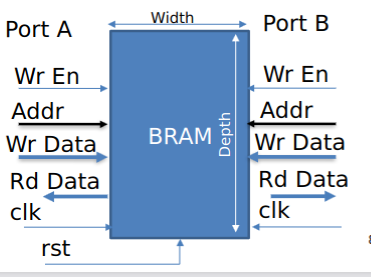
\includegraphics[width=0.6\textwidth]{images/BRAM.png}
\end{center}

Dual port configuration allows each port to run in different
clock frequencies.
One operation at a time (read or write at the same address.)

The smart thing about using dual port is that you can read
and write at the same time at different addresses.
